
In this section, we will implement the following machine learning algorithms:

\begin{enumerate}
    \item The Perceptron algorithm
    \item Support Vector Machines (SVMs) using the Pegasos algorithm
    \item Regularized logistic classification (i.e., the Pegasos objective function with logistic loss instead of hinge loss)
\end{enumerate}

In addition, we will attempt to evaluate these models with proper hyper-parameter optimization, reporting the training and test errors.

% ------------------------------------------------------
\section{Perceptron}

We know that a linear predictor for $\mathcal{X} \in \mathbb{R}^d$ is a function $h: \mathbb{R}^d \rightarrow \mathbb{R}$ defined as $h(x) = f(w^Tx)$ for some $w \in \mathbb{R}^d$, where $f: \mathbb{R} \rightarrow \mathbb{R}$ is often referred to as an \textit{activation function}. In linear classification tasks, we typically use $h(x) = \text{sgn}(w^Tx)$, where:
\begin{equation}
    \text{sgn}(z) = \begin{cases}
                        1 & \text{if } z > 0 \\
                        -1 & \text{otherwise}
                    \end{cases}
\end{equation}
In this case, the \textit{zero-one} loss $\mathbb{I}\{h(x_t) \neq y_t\}$ can be written as $\mathbb{I}\{y_t w^T x_t \leq 0 \}$. It should be noted that finding an efficient implementation of Empirical Risk Minimization (ERM) for linear classifiers using zero-one loss is unlikely, and the decision problem of finding $h_S$ is NP-complete, even in the case of binary features.

However, in the linearly separable case, there exists at least a solution which can be found in polynomial time to solve the ERM problem, for which we can use the \textit{Perceptron} algorithm for linear classifiers.

The Perceptron algorithm is a linear binary classifier that iteratively adjusts its weights based on the input features and the misclassified predictions, trying to find a homogeneous separating hyperplane which always terminates on linearly separable cases. It can also be seen as a single unit of an artificial neural network, where in the single layer case it's only capable of learning linearly separable patterns.

The general structure of a single Perceptron is illustrated in Figure~\ref{fig:perceptron}.

\begin{figure}[h]
    \centering
    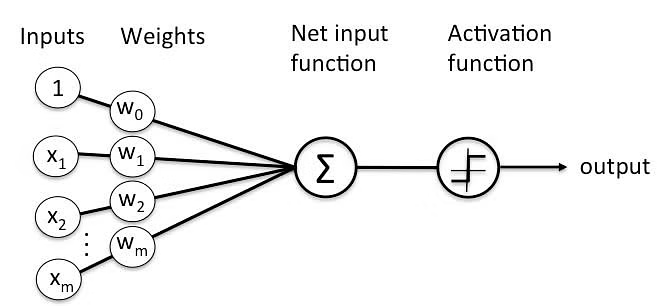
\includegraphics[width=0.7\linewidth]{images/perceptron.png}
    \caption{Perceptron Structure}
    \label{fig:perceptron}
\end{figure} \vspace{10pt}

We will implement the Perceptron, according to the following pseudo-code:

\begin{algorithm}[H]
    \SetAlgoLined
    \DontPrintSemicolon
    \caption{The Perceptron algorithm (for the linearly separable case)} \vspace{4pt}
    \KwIn{Training set $(x_1, y_1), \dots, (x_m, y_m) \in \mathbb{R}^d \times \{-1, 1\}$}
    Initialize $\boldsymbol{w} = (0, \dots, 0)$\\
    \While{true} {  
        \For(\ \text{(epoch)}){$i = 1, \dots, m$}{
            \uIf{$y_t \boldsymbol{w}^{\top}\boldsymbol{x}_t \leq 0$}{
                $\boldsymbol{w} \leftarrow \boldsymbol{w} + y_t \boldsymbol{x}_t$\ \text{(update)}\\ 
            }    
        }
        \uIf{no update in last epoch} {
            \textbf{break}
        } 
   }
    % \Return{$k$}
   \KwOut{$\boldsymbol{w}$}
\end{algorithm}\vspace{4pt}
        
Appendix~\ref{appendix:perceptron} includes the Python implementation of the Perceptron algorithm. The hyper-parameter \texttt{weight\_init} was included to test the effect of initializing the weights with zeros as opposed to the random initialization. Additionally, the \texttt{bias} term was also included to check it's effectiveness in the training procedure.

Using the \texttt{NestedCV} module, we attempted to tune the hyper-parameters, according to the grid provided as \texttt{param\_grid = \{'weight\_init': ['zeros', 'random'], 'bias': [True, False], 'max\_epochs': [20, 50, 120]\}}. According to the best hyper-parameter combination on the validation set, the model was re-trained on the whole training set and evaluated using the test set. Overall, the hyper-parameter optimization took \texttt{5min 10s} to be completed.

On average, the training set achieved an accuracy of \texttt{67.38\%}, precision of \texttt{69.74\%}, and recall of \texttt{59.06\%}, while the average test results were accuracy of \texttt{67.23\%}, precision \texttt{69.92\%}, and recall \texttt{58.95\%}. Therefore, the Perceptron model's accuracy on both the training and test set hovers around \texttt{65-70\%} and it does not show improvement with hyper-parameter tuning after a certain point. This fact suggests that we suffer from a mild underfitting, and the data may not be linearly separable.

Underfitting occurs when the model is too simple to capture the underlying patterns in the data. The Perceptron algorithm is a linear classifier, meaning it can only find a linear decision boundary to separate the classes. If the data is not linearly separable (i.e., the classes cannot be separated by a straight line in the feature space), the Perceptron won't be able to achieve high accuracy and the chosen features are insufficient to draw a clear linear boundary, which leads to underfitting.

In later chapters we will try to examine this hypothesis by both discussing the effect of adding polynomial features to the dataset and applying a kernel trick, checking if the model's performance improves significantly. If it does, then this is a strong indication that the original data was not linearly separable.

% ------------------------------------------------------
\section{Pegasos for SVM}

In general, the SVM optimization problem can be defined as:

\begin{itemize}
    \item For a given training set $(\boldsymbol{x}_1, y_1), \dots, (\boldsymbol{x}_m, y_m) \in \mathbb{R}^d \times \{-1, 1\}$ which is \textbf{linearly separable}, SVM outputs the linear classifier corresponding to the unique solution $\boldsymbol{w}^* \in \mathbb{R}^d$ of the \textit{convex optimization problem} with linear constraints defined as:
    \begin{equation}
        \underset{\boldsymbol{w} \in \mathbb{R}^d}{\min}\ \frac{1}{2} \Vert \boldsymbol{w} \Vert^2, \quad \text{such that} \quad y_t \boldsymbol{w}^\top \boldsymbol{x}_t \geq 1 \quad \text{for} \quad t = 1, \dots, m
    \end{equation}
    We can also say $\boldsymbol{w}^{*}$ geometrically corresponds to the \textit{maximum margin} separating hyperplane, and the maximum margin separator $\boldsymbol{u}^{*}$ is a solution to:
    \begin{equation}
        \underset{\boldsymbol{u} : \Vert \boldsymbol{u} \Vert = 1}{\max} \underset{t}{\min} \ y_t \boldsymbol{u}^\top \boldsymbol{x}_t
    \end{equation}

    \item For a given training set $(\boldsymbol{x}_1, y_1), \dots, (\boldsymbol{x}_m, y_m) \in \mathbb{R}^d \times \{-1, 1\}$ which is \textbf{not linearly separable}, the constraints can be satisfied up to a certain level called \textit{slack variables} $\xi = (\xi_1, \dots, \xi_m)$, measuring how much each margin constraint is violated by a potential solution $\boldsymbol{w}$. The average of these violations is then added to the objective function of the SVM, and a \textit{regularization} parameter $\lambda > 0$ is introduced to balance the two terms. Finally, we get:
    \begin{equation}
        \underset{(\boldsymbol{w}, \boldsymbol{\xi}) \in \mathbb{R}^{d+m}}{\min} \quad  \frac{\lambda}{2} \Vert \boldsymbol{w} \Vert^2 + \frac{1}{m} \sum_{t = 1}^m \xi_t \hspace{15pt}
        \text{s.t. for } t = 1, \dots, m \hspace{15pt}
        \begin{cases}
            y_t \boldsymbol{w}^\top \boldsymbol{x}_t \geq 1 - \xi_t \\
            \xi_t \geq 0
        \end{cases}
    \end{equation}
    Considering the constraints on slack variables, to minimize each $\xi_t$ we can set:
    \begin{equation}
        \xi_t =
        \begin{cases}
            1 - y_t \boldsymbol{w}^\top \boldsymbol{x}_t & \text{if} \ y_t \boldsymbol{w}^\top \boldsymbol{x}_t < 1 \\                
            0 & \text{otherwise}
        \end{cases}
        = \left[1 - y_t \boldsymbol{w}^\top \boldsymbol{x}_t \right]_+
        = \underbrace{h_{t}(\boldsymbol{w})}_{\text{hinge loss}}
    \end{equation}
    So, the SVM problem can be reformulated as:
    \begin{equation}
        \underset{\boldsymbol{w} \in \mathbb{R}^d}{\min} \ \underbrace{\frac{\lambda}{2} \Vert \boldsymbol{w} \Vert^2 + \frac{1}{m} \sum_{t = 1}^m h_{t}(\boldsymbol{w})}_{F(\boldsymbol{w})}
    \end{equation}
\end{itemize}

\textbf{Pegasos} is an instance of stochastic gradient descent (SGD) over online gradient descent (OGD) on SVM objective function, which is applied on $\lambda$-strongly convex functions to the set of losses $\ell_1,\dots,\ell_m$, where $\ell_t(w) = h_t(w) + \frac{\lambda}{2} \|w\|^2$, run over a sequence of examples randomly drawn from the training set, aiming to minimize $F$ which is described as:
\begin{equation}
    F(w) = \frac{1}{m} \sum_{t=1}^{m} \ell_t(w)
\end{equation}

Fixing a realization of random variables $s_1,\dots,s_t$ and $\eta_t = \frac{1}{\lambda t}$, we have:
\begin{equation}
    \nabla \ell_{s_t} (w_t) = -y_{s_t} x_{s_t} \mathbb{I} \{ h_{s_t}(w_t) > 0 \} + \lambda w_t \\
\end{equation}

We will implement the Pegasos for SVM, according to the following pseudo-code:

\begin{algorithm}[H]
    \SetAlgoLined
    \DontPrintSemicolon
    \caption{Pegasos for SVM} \vspace{4pt}
    \KwIn{Training set $S$, number of rounds $T$, regularization coefficient $\lambda > 0$}
    Initialize $\boldsymbol{w}_1 = (0, \dots, 0)$\\
    \For{$t = 1, \dots, T$}{
        Draw uniformly at random $Z_t \sim \{1, \dots, m\}$, obtaining $(\boldsymbol{x}_{Z_t}, y_{Z_t})$ from $S$\\
        Set $\boldsymbol{w}_{t+1} \leftarrow \boldsymbol{w}_t - \eta_t \nabla \ell_{Z_t}(\boldsymbol{w}_t)$ \\
    }
    \KwOut{$\boldsymbol{\bar{w}} = \frac{1}{T} \sum_{t=1}^{T} \boldsymbol{w}_t$}
\end{algorithm}

The implementation for \texttt{PegasosSVM} module is provided at the Appendix~\ref{appendix:pegasos}. This class contains both hinge and logistic loss functions since the majority of the code is shared with the \textit{logistic classification} algorithm. Hence, the hyper-parameter \texttt{loss} can be defined as either \texttt{"hinge"} or \texttt{"logistic"}, \texttt{T} denotes the number of rounds, and \texttt{lambda\_param} controls the regularization coefficient.

According to the \texttt{param\_grid = \{'loss': ['hinge'], 'T': [1000, 2000, 5000], 'lambda\_param': [0.001, 0.01, 0.1]\}} for the \texttt{NestedCV} module, the hyper-parameters were tuned, where for this evaluation we fixed the loss to be explicitly \texttt{'hinge'}. The best hyperparameter combination by the majority of folds on the validation set was selected as \texttt{\{'loss': 'hinge', 'T': 5000, 'lambda\_param': 0.1\}}, which was further re-trained accordingly on the training set, and evaluated via test set. The hyper-parameter optimization only took \texttt{17s} in total.

The training set achieved an average accuracy of \texttt{71.63\%}, a precision of \texttt{70.43\%}, and a recall of \texttt{71.23\%}. In comparison, the test set produced an average accuracy of \texttt{71.57\%}, a precision of \texttt{70.39\%}, and a recall of \texttt{71.16\%}. Both the training and test sets consistently yield results around \texttt{70\%}. Despite efforts in hyper-parameter optimization, the results cannot be further improved after a certain point, likely due to the model's simplicity which limits its ability to capture complex patterns, similar to the evaluation seen in the Perceptron model.

% ------------------------------------------------------
\section{Regularized Logistic Classification}

The zero-one loss can be shown to be NP-hard, being unlikely to be solved using a polynomial time algorithm. In addition, the loss function is non-smooth and non-convex, where small changes in $w$ can change the loss by a lot, hence we use convex approximations to the zero-one loss. While the SVM is based on hinge loss, the logistic regression model instead uses a loss function called \textit{log-loss}, which has a real gradient (not just a sub-gradient like hinge) and a smooth shape.

In order to implement the regularized logistic classification, we should adopt the Pegasos objective function along with \textit{logistic loss}. Since the structures of the two algorithms are quite similar, it makes sense to modify the existing \texttt{PegasosSVM} class from the previous section to accommodate both types of loss functions, including the logistic loss which is defined as:
\begin{equation}
    \ell(y, \hat{y}) = \log_2(1 + e^{-y\hat{y}})
\end{equation}

Given the $t$-th example of the training set $S = \{(x_1,y_1),\dots,(x_m,y_m)\}$ in the case of linear models where $\hat{y} = g(\boldsymbol{x}) = \boldsymbol{w}^\top \boldsymbol{x}$ and $w \in \mathbb{R}^d$, the logistic loss for logistic regression can be written as below, where a regularization term is often added to enforce stability and avoid overfitting (Regularized LR):
\begin{equation}
    \ell_t (w) = \log_2(1+e^{-y_t w^\top x_t}) + \frac{\lambda}{2} \|w\|^2
\end{equation}

Fixing a realization of random variables $s_1,\dots,s_t$ and $\eta_t = \frac{1}{\lambda t}$, we have:
\begin{equation}
    \nabla \ell_{s_t} (w_t) = \frac{-\sigma\left( -y_{s_t} w_t^\top x_{s_t} \right)}{\ln 2} y_{s_t} x_{s_t} + \lambda w_t
\end{equation}

where the function $\sigma: \mathbb{R} \rightarrow \mathbb{R}$, called logistic, is defined as:
\begin{equation}
    \sigma(z) = \frac{1}{1 + e^{-z}} \in (0,1)
\end{equation}

Again, the implementation for \texttt{PegasosSVM} module containing the logistic loss can be found in Appendix~\ref{appendix:pegasos}. Given the \texttt{param\_grid = \{'loss': ['logistic'], 'T': [1000, 2000, 5000], 'lambda\_param': [0.001, 0.01, 0.1]\}} for the \texttt{NestedCV} module, the hyper-parameter tuning was performed, where the \texttt{'logistic'} loss was explicitly fixed for evaluation. All the folds confirmed that \texttt{\{'lambda\_param': 0.1\}} is the best choice for regularization parameter, while the choice of \texttt{T} varied by folds on the validation from one another, re-training on the training set and evaluating on the test set accordingly. The whole hyper-parameter optimization process only took around \texttt{17s} to complete.

The training set showed an average accuracy of \texttt{71.57\%}, with a precision of \texttt{70.38\%} and a recall of \texttt{71.09\%}. For the test set, the average accuracy was \texttt{71.21\%}, precision \texttt{70.07\%}, and recall \texttt{70.59\%}. The results are again somehow similar to the previous algorithms, stuck around \texttt{70\%} accuracy, and there seems to be underfitting due to the simplicity of the model.